\documentclass[12pt]{article}
\usepackage[utf8]{inputenc}
\usepackage[spanish]{babel}
\decimalpoint
\usepackage{mathtools}
\usepackage{amsmath}
\usepackage{amsthm}
\usepackage{amssymb}
\usepackage{graphicx}
\usepackage[margin=0.9in]{geometry}
\usepackage{fancyhdr}
\usepackage[inline]{enumitem}
\usepackage{float}
\usepackage{cancel}
\usepackage{bigints}
\usepackage{color}
\usepackage{xcolor}
\usepackage{listingsutf8}
\usepackage{algorithm}
\usepackage{tocloft}
\usepackage[none]{hyphenat}
\usepackage{graphicx}
\usepackage{grffile}
\usepackage{tabularx}
\usepackage[nottoc,notlot,notlof]{tocbibind}
\usepackage{times}
\usepackage{color}
\definecolor{gray97}{gray}{.97}
\definecolor{gray75}{gray}{.75}
\definecolor{gray45}{gray}{.45}
\renewcommand{\cftsecleader}{\cftdotfill{\cftdotsep}}
\pagestyle{fancy}
\setlength{\headheight}{15pt} 
\lhead{Autómata}
\rhead{\thepage}
\lfoot{ESCOM-IPN}
\renewcommand{\footrulewidth}{0.5pt}
\setlength{\parskip}{0.5em}
\newcommand{\ve}[1]{\overrightarrow{#1}}
\newcommand{\abs}[1]{\left\lvert #1 \right\lvert}
\date{ 22 de Marzo 2018}
\title{Automata}
\author{Reporte 3}

\definecolor{pblue}{rgb}{0.13,0.13,1}
\definecolor{pgreen}{rgb}{0,0.5,0}
\definecolor{pred}{rgb}{0.9,0,0}
\definecolor{pgrey}{rgb}{0.46,0.45,0.48}
\lstset{tabsize=1}

\usepackage{listings}
\lstset{ frame=Ltb,
framerule=0pt,
aboveskip=0.5cm,
framextopmargin=3pt,
framexbottommargin=3pt,
framexleftmargin=0.4cm,
framesep=0pt,
rulesep=.4pt,
backgroundcolor=\color{gray97},
rulesepcolor=\color{black},
%
stringstyle=\ttfamily,
showstringspaces = false,
basicstyle=\small\ttfamily,
commentstyle=\color{gray45},
keywordstyle=\bfseries,
%
numbers=left,
numbersep=15pt,
numberstyle=\tiny,
numberfirstline = false,
breaklines=true,
}

% minimizar fragmentado de listados
\lstnewenvironment{listing}[1][]
{\lstset{#1}\pagebreak[0]}{\pagebreak[0]}

\lstdefinestyle{consola}
{basicstyle=\scriptsize\bf\ttfamily,
backgroundcolor=\color{gray75},
}

\lstdefinestyle{Java}
{language=Java,
}

%%%%%%%%%%%%%%%%%%%%%

\lstdefinestyle{customc}{
  belowcaptionskip=1\baselineskip,
  breaklines=true,
  frame=L,
  xleftmargin=\parindent,
  language=C,
  showstringspaces=false,
  basicstyle=\footnotesize\ttfamily,
  keywordstyle=\bfseries\color{green!40!black},
  commentstyle=\itshape\color{purple!40!black},
  identifierstyle=\color{blue},
  stringstyle=\color{orange},
}

\lstdefinestyle{customasm}{
  belowcaptionskip=1\baselineskip,
  frame=L,
  xleftmargin=\parindent,
  language=[x86masm]Assembler,
  basicstyle=\footnotesize\ttfamily,
  commentstyle=\itshape\color{purple!40!black},
}

\lstset{escapechar=@,style=customc}

%Permite crear columnas en el documento
\usepackage{multicol} 
\usepackage{color}
\usepackage{comment}
\newcommand{\tabitem}{~~\llap{\textbullet}~~}
\newcommand{\subtabitem}{~~~~\llap{\textbullet}~~}

\bibliographystyle{IEEEtran}
\begin{document}
		\begin{titlepage}
			\begin{center}
				
				% Upper part of the page. The '~' is needed because \\
				% only works if a paragraph has started.
				
				\noindent
				\begin{minipage}{0.5\textwidth}
					\begin{flushleft} \large
						\includegraphics[width=0.3\textwidth]{../ipn.png}
					\end{flushleft}
				\end{minipage}%
				\begin{minipage}{0.55\textwidth}
					\begin{flushright} \large
						\includegraphics[width=0.7\textwidth]{../escom.png}
					\end{flushright}
				\end{minipage}
				
				\textsc{\LARGE Instituto Politécnico Nacional}\\[0.5cm]
				
				\textsc{\Large Escuela Superior de Cómputo}\\[1cm]
				
				% Title
				
				{ \huge Práctica 3 - Autómata \\[1cm] }
				
				{ \Large Unidad de aprendizaje: Teoría computacional} \\[1cm]
				
				{ \Large Grupo: 2CM4 } \\[1cm]
				
				\noindent
				\begin{minipage}{0.5\textwidth}
					\begin{flushleft} \large
						\emph{Alumno(a):}\\
						
						\begin{tabular}{ll}
					     Nicolás Sayago Abigail\\
					\end{tabular}
					\end{flushleft}
				\end{minipage}%
				\begin{minipage}{0.5\textwidth}
					\begin{flushright} \large
						\emph{Profesor(a):} \\
						Sanchez García Luz María  \\
					\end{flushright}
				\end{minipage}
				
				\vfill
				
				% Bottom of the page
				{\large 22 de Marzo de 2018}
			\end{center}
		\end{titlepage}
	
	\tableofcontents
	\newpage
	% \\\\\\\\\\\\\\\\\\\\\\\\\\\\\\\\\\\\\\\\\\\\\\\\\\\\\\\\\\\\
	% \\\\\\\\\\\\\\\\\\\\\\\ INTRODUCCION \\\\\\\\\\\\\\\\\\\\\\\
	% \\\\\\\\\\\\\\\\\\\\\\\\\\\\\\\\\\\\\\\\\\\\\\\\\\\\\\\\\\\\

	\section{Introducción}
	En la siguiente práctica se implementara el autómata de una expresión regular en el lenguaje de programación de JAVA.
	La expresión regular sera de un número de boleta que pertenece a un Sistema Administrativo y Escolar 
	de Educación Básica (SAEEB), que está siendo desarrollado. Dicha expresión regular ya fue explicada en el reporte 2.

	A lo largo del documento usaremos la palabra \textbf{Autómata}, por lo cual tenemos que definir
	¿Qué es un autómata?.

	\noindent\textbf{Autómata} \\
	La palabra autómata viene del griego \textsl{automatos} que significa espontáneo o con movimiento propio. 

	\noindent\textbf{Autómata programable}\\
	En 1938 el matemático norteamericano Claude Elwood Shannon, estableció las bases de la 
	aplicación de la lógica matemática para los circuitos combinatorios, y secuenciales, construidos
	a bases de relés y más adelante con otros dispositivos de vacío y estado solido.
	Los autómatas son sistemas capaces de transmitir información. En amplio sentido, todo sistema que
	acepta señales de su entorno y, como resultado, cambia de estado y transmite otras señales al medio,
	puede considerarse un autómata.
	No tiene sus propios movimientos, sino que estos parecen ser de robot.

	\noindent\textbf{Teoría de Autómatas} \\
	Para la teoría de la computación existe un área de estudio conocida como la teoría de autómatas, 
	esta estudia las máquinas abstractas y los problemas que éstas son capaces de resolver.
	Un autómata es un modelo matemático para una máquina de estados, que, dada una entrada de 
	símbolos, salta a través de una serie de estados de acuerdo a una función de transición produciendo 
	salidas. La teoría de autómatas está estrechamente relacionada con la teoría del lenguaje formal ya que los 
	autómatas son clasificados a menudo por la clase de lenguajes formales que son capaces de reconocer.

	El autómata recibe los símbolos de entrada, uno detrás de otro, es decir secuencialemente.

	\noindent\textbf{Estado de un autómata} \\
	Es toda la información necesaria en eun momento dado, para poder deducir, dado un símbolo de entrada 
	en ese momento, cual será el símbolo de salida.  

	El autómata tendrá un determinado número de estados(pudiendo ser infinitos), y se encontrará en uno 
	u otro según sea la historia de símbolos que le han llegado.

	\newpage
	% \\\\\\\\\\\\\\\\\\\\\\\\\\\\\\\\\\\\\\\\\\\\\\\\\\\\\\\\\\\\\\\\\\\\\\\\\\
	% \\\\\\\\\\\\\\\\\\\\\\\ PLANTEAMIENTO DEL PROBLEMA \\\\\\\\\\\\\\\\\\\\\\\
	% \\\\\\\\\\\\\\\\\\\\\\\\\\\\\\\\\\\\\\\\\\\\\\\\\\\\\\\\\\\\\\\\\\\\\\\\\\

	\section{Planteamiento del problema}
	Recordando que para esta práctica delimitamos el número de boleta para un alumno del Estado de México.
	Así que diseñamos la solución para implementar el autómata definido por lo siguiente:

	\begin{itemize}
		\item Niños que hayan ingresado en los años 2014-2017.								
		\item Que la escuela pertenezca a la entidad federativa Estado de México. 			
		\item Que sea de uno de los 125 municipios de esa entidad federativa.				
		\item Pertenezca a una de las escuelas en ese municipio (0-99)						
		\item Puede ser Alumno o Docente, siendo identificados con A y D respectivamente.	
		\item Número de usuario dado por 3 números y una letra.	(Identificador).							
		\item Tiene un total de 16 caracteres.
	\end{itemize}

	\begin{figure}[H]
	        \centering
	        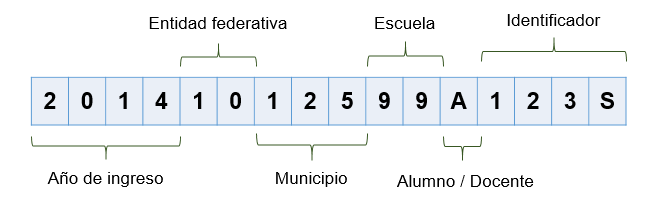
\includegraphics[scale=0.9]{Practica2/Estructura.PNG}
	\end{figure}
	\begin{multicols}{2}[Algunos ejemplos son:]
		Cadenas validas son:
		\begin{itemize}
			\item 20141012599A123A
			\item 20141012599D144A
			\item 20151000198A126R
			\item 20171003474A112D
		\end{itemize}
		\columnbreak
		Cadenas no validas:
		\begin{itemize}
			\item 20181312599S123A12  
			\item 20171013515D014S    
			\item 20141012599A131$<$  
			\item 20131012610D123A  
			\end{itemize}
	\end{multicols}
	\newpage

	% \\\\\\\\\\\\\\\\\\\\\\\\\\\\\\\\\\\\\\\\\\\\\\\\\\\\\\\\\\\\\\\\\\\\\
	% \\\\\\\\\\\\\\\\\\\\\\\ DISEÑO DE LA SOLUCION \\\\\\\\\\\\\\\\\\\\\\\
	% \\\\\\\\\\\\\\\\\\\\\\\\\\\\\\\\\\\\\\\\\\\\\\\\\\\\\\\\\\\\\\\\\\\\\\

	\section{Diseño de la solución}

	A continuación mostraré el diseño que se tiene para implementar la solución, dados
	los requerimientos expresados antes. \\
	El autómata es:

	\begin{figure}[H]
	        \centering
	        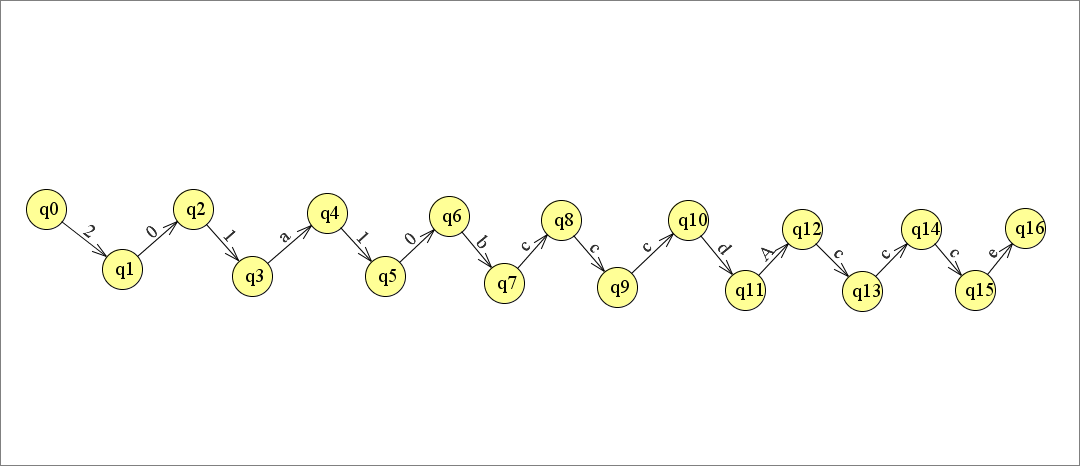
\includegraphics[scale=0.4]{Practica3/automata.PNG}
	\end{figure}

	Donde:
	\begin{itemize}
		\item \textbf{a}: Números del 4 al 7
		\item \textbf{b}: Número 0 o 1
		\item \textbf{c}: Números del 0 al 9
		\item \textbf{d}: Números del 1 al 9
		\item \textbf{e}: Letras de la A a la Z
	\end{itemize}

	\newpage
	% \\\\\\\\\\\\\\\\\\\\\\\\\\\\\\\\\\\\\\\\\\\\\\\\\\\\\\\\\\\\\\\\\\\\\\\\\\\\\
	% \\\\\\\\\\\\\\\\\\\\\\\ IMPLEMENTACION DE LA SOLUCION \\\\\\\\\\\\\\\\\\\\\\\
	% \\\\\\\\\\\\\\\\\\\\\\\\\\\\\\\\\\\\\\\\\\\\\\\\\\\\\\\\\\\\\\\\\\\\\\\\\\\\\

	\section{Implementación de la solución}

	De forma general el programa esta estructurado de tal forma que se introduce una cadena, 
	al dar click al boton \textbf{OK} el programa empieza a validar cada uno de los estados.

	Existen dos archivos, el primero llamado \textbf{Main.java} y el segundo \textbf{Boleta.java}.\\
	A continuación se muestra cada parte de ellos fundamental para que el programa funcione.

	\textbf{IMPLEMENTACIÓN DEL MAIN}
	\begin{lstlisting}[style=Java]
// Recibe los eventos al presionar el boton 
public void actionPerformed(ActionEvent e)
{
	JButton b = (JButton)e.getSource();
	// Si se presiona el boton OK
	if(b == Enviar)
	{
		// Se limpia la entrada
		AreaSalida.setText("");
		// Se envía la boleta 
		Automata.setBoleta(Cadena.getText());
		// Se inicia el proceso de evaluar estados
		Automata.Iniciar();
		// Se verifica si la cadena es valida
		if(Automata.Verificar())
			AreaSalida.setText(AreaSalida.getText() + " Cadena Valida\r\n");
		else
			AreaSalida.setText(AreaSalida.getText() + " Cadena NO Valida\r\n");
	}
}
	\end{lstlisting}			

	\textbf{IMPLEMENTACIÓN DE LA CLASE BOLETA}
	\begin{itemize}
		\item[$\overrightarrow$] \textbf{Métodos principales y necesarios}

		\begin{lstlisting}[style=Java]
// Metodo constructor
public Boleta(String NumBoleta, JTextArea auxText)
{
	this.NumBoleta = NumBoleta;
	this.auxText = auxText;
}
		\end{lstlisting}

		\begin{lstlisting}[style=Java]
// Obtiene la boleta
public void setBoleta(String NumBoleta)
{
	this.NumBoleta = NumBoleta;
}
		\end{lstlisting}

\newpage
	
		\begin{lstlisting}[style=Java]
/* Método que permite verificar si la cadena cumple 
	con la longitud requerida, en este caso 16. */
public boolean Verificar()
{
	if(i==16)
		return true;
	else
		return false;
}
		\end{lstlisting}

		\begin{lstlisting}[style=Java]
/* Método que inicia la verificación de estados */
public void Iniciar()
{
	i = 0; // Se inicializa la variable contadora
	qo(); // Empieza el estado 0
}
		\end{lstlisting}
		

		\item[$\overrightarrow$] \textbf{Estado CERO}

		\begin{lstlisting}[style=Java]
// Método del ESTADO 0 
public void qo()
{
	auxText.setText(auxText.getText()+"Q0\r\n");
	if(i< NumBoleta.length())
	{
		// Verifica que sea un número 2
		if('2'==NumBoleta.charAt(i))
			i++; q1();
	}
}	
		\end{lstlisting}

		\item[$\overrightarrow$] \textbf{Estado UNO}

		\begin{lstlisting}[style=Java]
// Método del ESTADO 1
public void q1()
{
	auxText.setText(auxText.getText()+"Q1\r\n");
	if(i< NumBoleta.length())
	{
		// Verifica que sea un número 0
		if('0'==NumBoleta.charAt(i))
			i++; q2();
	}
}
		\end{lstlisting}
\newpage

		\item[$\overrightarrow$] \textbf{Estado DOS}

		\begin{lstlisting}[style=Java]
// Método del ESTADO 2
public void q2()
{
	auxText.setText(auxText.getText() + "Q2\r\n");
	if(i < NumBoleta.length())
	{
		// Verifica que sea un número 1
		if('1'==NumBoleta.charAt(i))
			i++; q3();
	}	
}
		\end{lstlisting}

		\item[$\overrightarrow$] \textbf{Estado TRES}

		\begin{lstlisting}[style=Java]
// Método del ESTADO 3
public void q3()
{
	auxText.setText(auxText.getText() + "Q3\r\n");
	if(i < NumBoleta.length())
	{
		int num = Integer.parseInt(""+NumBoleta.charAt(i));
		// Cumple el rango de [4-7]
		if( (num > 3) && (num < 8) )
		{
			i++; 
			q4();
		}
	}
}
		\end{lstlisting}

		\item[$\overrightarrow$] \textbf{Estado CUATRO}

		\begin{lstlisting}[style=Java]
// Método del ESTADO 4
public void q4()
{
	auxText.setText(auxText.getText() + "Q4\r\n");
	if(i < NumBoleta.length())
	{
		// Verifica que sea un número 1
		if('1'==NumBoleta.charAt(i))
			i++; q5();
	}	
}
		\end{lstlisting}
\newpage

		\item[$\overrightarrow$] \textbf{Estado CINCO}

		\begin{lstlisting}[style=Java]
// Método del ESTADO 5
public void q5()
{
	auxText.setText(auxText.getText() + "Q5\r\n");
	if(i < NumBoleta.length())
	{
		// Verifica que sea un número 0
		if('0'==NumBoleta.charAt(i))
			i++; q6();
	}	
}
		\end{lstlisting}

		\item[$\overrightarrow$] \textbf{Estado SEIS}

		\begin{lstlisting}[style=Java]
// Método del ESTADO 6
public void q6()
{
	auxText.setText(auxText.getText() + "Q6\r\n");
	if(i < NumBoleta.length())
	{
		int num = Integer.parseInt(""+NumBoleta.charAt(i));
		// Cumple el rango de [0-1]
		if( (num >= 0) && (num < 2))
			i++; q7();
	}
}
		\end{lstlisting}

		\item[$\overrightarrow$] \textbf{Estado SIETE}

		\begin{lstlisting}[style=Java]
// Método del ESTADO 7
public void q7()
{
	auxText.setText(auxText.getText() + "Q7\r\n");
	if(i < NumBoleta.length())
	{
		int num = Integer.parseInt(""+NumBoleta.charAt(i));
		int numAnt = Integer.parseInt(""+NumBoleta.charAt(i-1));
		if(numAnt == 0)
		{
			// Cumple el rango de [0-9]
			if( (num >= 0) && (num < 10))
				i++; q8();
		}
		else 
		{
			// Cumple el rango de [0-2]
			if( (num >= 0) && (num < 3))
				i++; q8();
		}
	}	
}
		\end{lstlisting}

\newpage
		\item[$\overrightarrow$] \textbf{Estado OCHO}

		\begin{lstlisting}[style=Java]
// Método del ESTADO 8
public void q8()
{
	auxText.setText(auxText.getText() + "Q8\r\n");
	if(i < NumBoleta.length() )
	{
		int num = Integer.parseInt(""+NumBoleta.charAt(i));
		// Cumple el rango de [0-9]
		if( (num >= 0) && (num < 10))
			i++; q9();
	}	
}
		\end{lstlisting}

		\item[$\overrightarrow$] \textbf{Estado NUEVE}

		\begin{lstlisting}[style=Java]
// Método del ESTADO 9
public void q9()
{
	auxText.setText(auxText.getText() + "Q9\r\n");
	if(i < NumBoleta.length())
	{
		int num = Integer.parseInt(""+NumBoleta.charAt(i));
		// Cumple el rango de [0-9]
		if( (num >= 0) && (num < 10))
			i++; q10();
	}	
}
		\end{lstlisting}

		\item[$\overrightarrow$] \textbf{Estado DIEZ}

		\begin{lstlisting}[style=Java]
// Método del ESTADO 10
public void q10()
{
	auxText.setText(auxText.getText() + "Q10\r\n");
	if(i < NumBoleta.length())
	{
		int num = Integer.parseInt(""+NumBoleta.charAt(i));
		// Cumple el rango de [1-9]
		if( (num >= 1) && (num < 10))
			i++; q11();
	}	
}
		\end{lstlisting}

		\newpage

		\item[$\overrightarrow$] \textbf{Estado ONCE}

		\begin{lstlisting}[style=Java]
// Método del ESTADO 11
public void q11()
{
	String letra1 = "A", letra2 = "D";
	char car = NumBoleta.charAt(i);
	auxText.setText(auxText.getText() + "Q11\r\n");
	if(i < NumBoleta.length())
	{
		if(String.valueOf(car).equals(letra1) || String.valueOf(car).equals(letra2))
			i++; q12();	
	}
}
		\end{lstlisting}

		\item[$\overrightarrow$] \textbf{Estado DOCE}

		\begin{lstlisting}[style=Java]
// Método del ESTADO 12
public void q12()
{
	auxText.setText(auxText.getText() + "Q12\r\n");
	if(i < NumBoleta.length())
	{
		int num = Integer.parseInt(""+NumBoleta.charAt(i));
		// Cumple el rango [0-9]
		if( (num >= 0) && (num < 10))
			i++; q13();
	}	
}
		\end{lstlisting}

		\item[$\overrightarrow$] \textbf{Estado TRECE}

		\begin{lstlisting}[style=Java]
// Método del ESTADO 13
public void q13()
{
	auxText.setText(auxText.getText() + "Q13\r\n");
	if(i < NumBoleta.length())
	{
		int num = Integer.parseInt(""+NumBoleta.charAt(i));
		// Cumple el rango [0-9]
		if( (num >= 0) && (num < 10))
			i++; q14();
	}	
}

		\end{lstlisting}
	\newpage

		\item[$\overrightarrow$] \textbf{Estado CATORCE}

		\begin{lstlisting}[style=Java]
// Método del ESTADO 14
public void q14()
{
	auxText.setText(auxText.getText() + "Q14\r\n");
	if(i < NumBoleta.length())
	{
		int num = Integer.parseInt(""+NumBoleta.charAt(i));
		// Cumple el rango [0-9]
		if( (num >= 0) && (num < 10))
			i++; q15();
	}	
}
		\end{lstlisting}

		\item[$\overrightarrow$] \textbf{Estado QUINCE}

		\begin{lstlisting}[style=Java]
// Método del ESTADO 15
public void q15()
{
	auxText.setText(auxText.getText() + "Q15\r\n");
	char[] abecedario;
	int j;
	if (i< NumBoleta.length())
	{
		abecedario = new char[26];
		for(j=0; j<26; j++)
			abecedario[j] = (char)('A' + j);
		for(j=0; j<26; j++)
		{
			if(NumBoleta.charAt(i) == abecedario[j])
				j=26; q16(); i++;	
		}
	}
}
		\end{lstlisting}

		\item[$\overrightarrow$] \textbf{Estado DIEZ Y SEIS}

		\begin{lstlisting}[style=Java]
	// Método del ESTADO 16 - FIN -
	public void q16()
	{
		auxText.setText(auxText.getText() + "Q16\r\n");
		if(NumBoleta.length()>16)
			i=17;
	}
		\end{lstlisting}

	\end{itemize}

\newpage

	% \\\\\\\\\\\\\\\\\\\\\\\\\\\\\\\\\\\\\\\\\\\\\\\\\\\\\\\\\\\\\\
	% \\\\\\\\\\\\\\\\\\\\\\\ FUNCIONAMIENTO \\\\\\\\\\\\\\\\\\\\\\\
	% \\\\\\\\\\\\\\\\\\\\\\\\\\\\\\\\\\\\\\\\\\\\\\\\\\\\\\\\\\\\\\

	\section{Funcionamiento}
	Primero que nada, mostramos la interfaz inicial. Observamos que el 
	usuario tiene la oportunidad de ingresar una cadena. Al dar click en el botón OK, se mostrarán los
	estados por los que pasa la cadena para mostrar si es una cadena valida o no.

	Se muestra \textbf{CADENA VALIDA} si la cadena que se ha ingresado cumple con el formato del número de boleta
	en caso contrario, se mostrará \textbf{CADENA NO VALIDA}.

	La pantalla inicial es la siguiente:
	
	\begin{figure}[H]
	        \centering
	        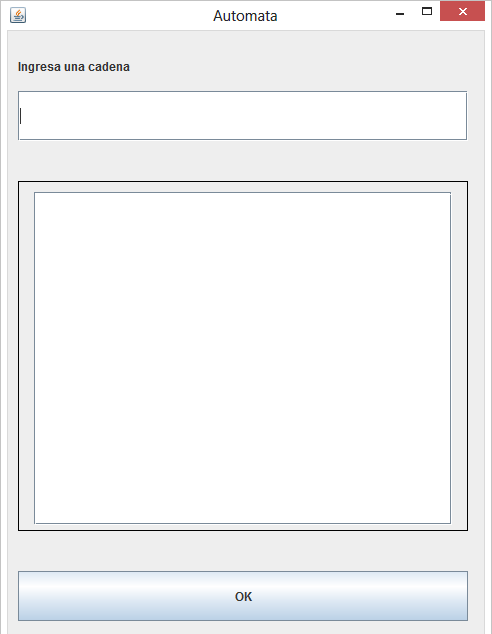
\includegraphics[scale=0.9]{Practica3/F_1.PNG}
	\end{figure}
	\newpage
	A continuación muestro ejemplos de \textbf{cadenas validas}: 
	\begin{figure}[H]
	        \centering
	        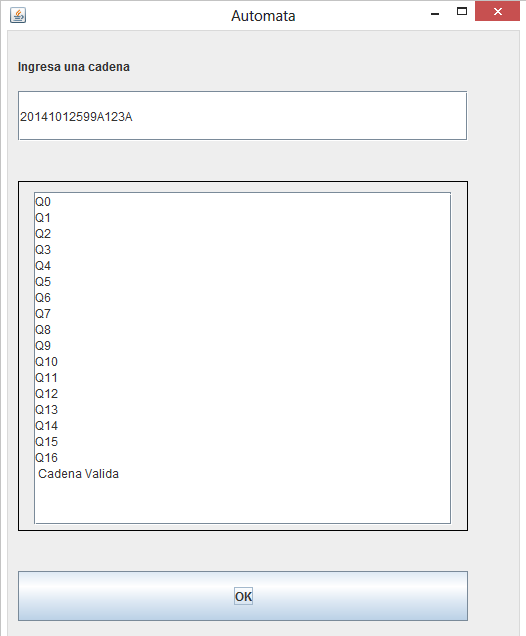
\includegraphics[scale=0.9]{Practica3/F_2.PNG}
	\end{figure}
	
	\begin{figure}[H]
	        \centering
	        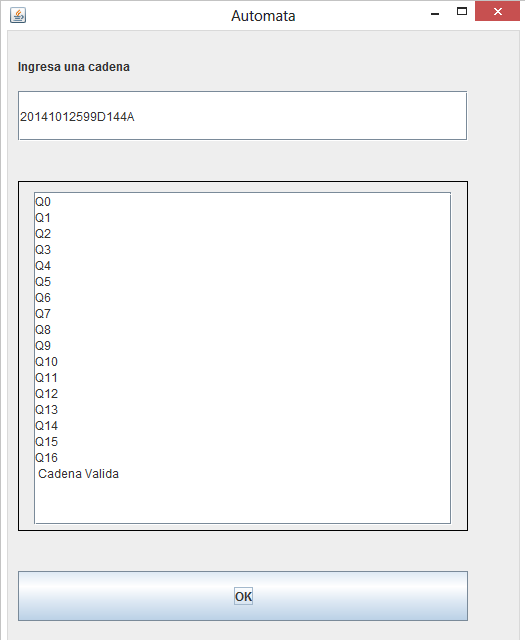
\includegraphics[scale=0.9]{Practica3/F_3.PNG}
	\end{figure}

	\begin{figure}[H]
	        \centering
	        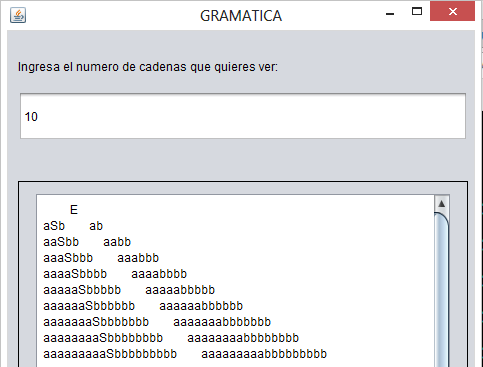
\includegraphics[scale=0.9]{Practica3/F_4.PNG}
	\end{figure}

	\begin{figure}[H]
	        \centering
	        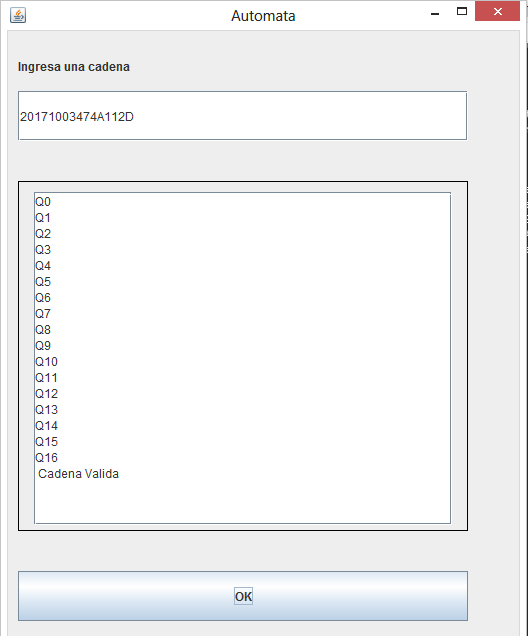
\includegraphics[scale=0.9]{Practica3/F_5.PNG}
	\end{figure}
	\newpage

	Ahora ejemplos de \textbf{cadenas no validas}:
	\begin{figure}[H]
	        \centering
	        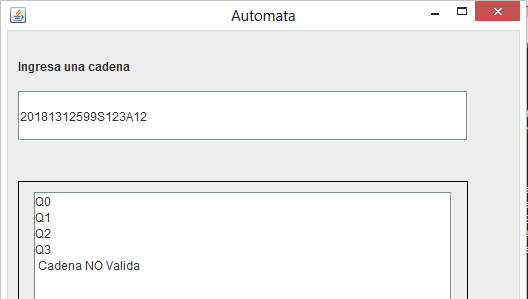
\includegraphics[scale=0.9]{Practica3/F_6.PNG}
	\end{figure}

	\begin{figure}[H]
	        \centering
	        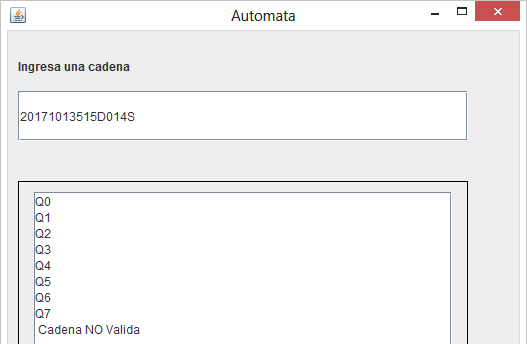
\includegraphics[scale=0.9]{Practica3/F_7.PNG}
	\end{figure}

	\begin{figure}[H]
	        \centering
	        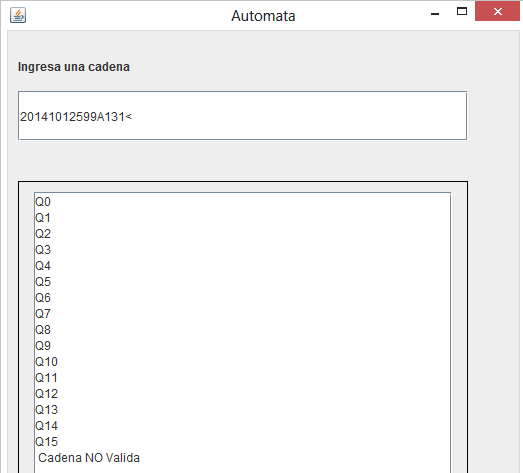
\includegraphics[scale=0.9]{Practica3/F_8.PNG}
	\end{figure}

	\begin{figure}[H]
	        \centering
	        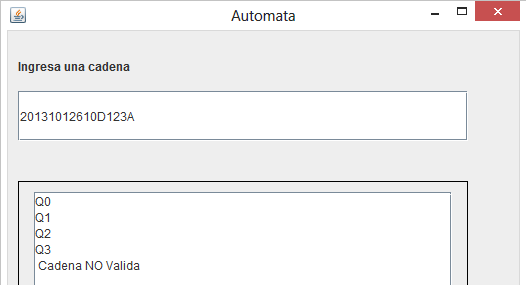
\includegraphics[scale=0.9]{Practica3/F_9.PNG}
	\end{figure}

	% \\\\\\\\\\\\\\\\\\\\\\\\\\\\\\\\\\\\\\\\\\\\\\\\\\\\\\\\\\\\
	% \\\\\\\\\\\\\\\\\\\\\\\ CONCLUSIONES \\\\\\\\\\\\\\\\\\\\\\\
	% \\\\\\\\\\\\\\\\\\\\\\\\\\\\\\\\\\\\\\\\\\\\\\\\\\\\\\\\\\\\
	\newpage
	\section{Conclusiones}

	Al terminar está práctica pude llevar a cabo la implementación del autómata que 
	esta basado en el número de boleta de un alumno del estado de México que cursa
	la escuela secundaria, dicho número de boleta esta propuesto desde la práctica 
	anterior. Especificamente, está práctica me ha ayudado a observar de manera más 
	directa como se comporta un autómata, y que es mejor programarlo por estados.

	Inicialmente mi idea era usar muchos \textsl{if} para que se validará la cadena,
	pero cuando iba a la mitad me di cuenta que estaba trabajando de más y que no 
	era la forma más eficiente de llevarlo a cabo, entonces hice la implementación
	que fue mostrada anteriormente. 


	% \\\\\\\\\\\\\\\\\\\\\\\\\\\\\\\\\\\\\\\\\\\\\\\\\\\\\\\\\\\\
	% \\\\\\\\\\\\\\\\\\\\\\\ BIBLIOGRAFIA \\\\\\\\\\\\\\\\\\\\\\\
	% \\\\\\\\\\\\\\\\\\\\\\\\\\\\\\\\\\\\\\\\\\\\\\\\\\\\\\\\\\\\

	 \nocite{ref1, ref2}
	\bibliography{referencias}
\end{document}